\documentclass{article}
\usepackage{graphicx} % Required for inserting images
\usepackage{tikz}
\usetikzlibrary{calc}

\title{12_45}
\author{zhi76.230 }
\date{May 2023}

% \begin{document}

% \maketitle
% https://tex.stackexchange.com/questions/222882/drawing-minimal-xy-axis
% \documentclass[tikz,border=2mm]{standalone}
\begin{document}
% https://tex.stackexchange.com/questions/15994/setting-unit-length-in-tikz
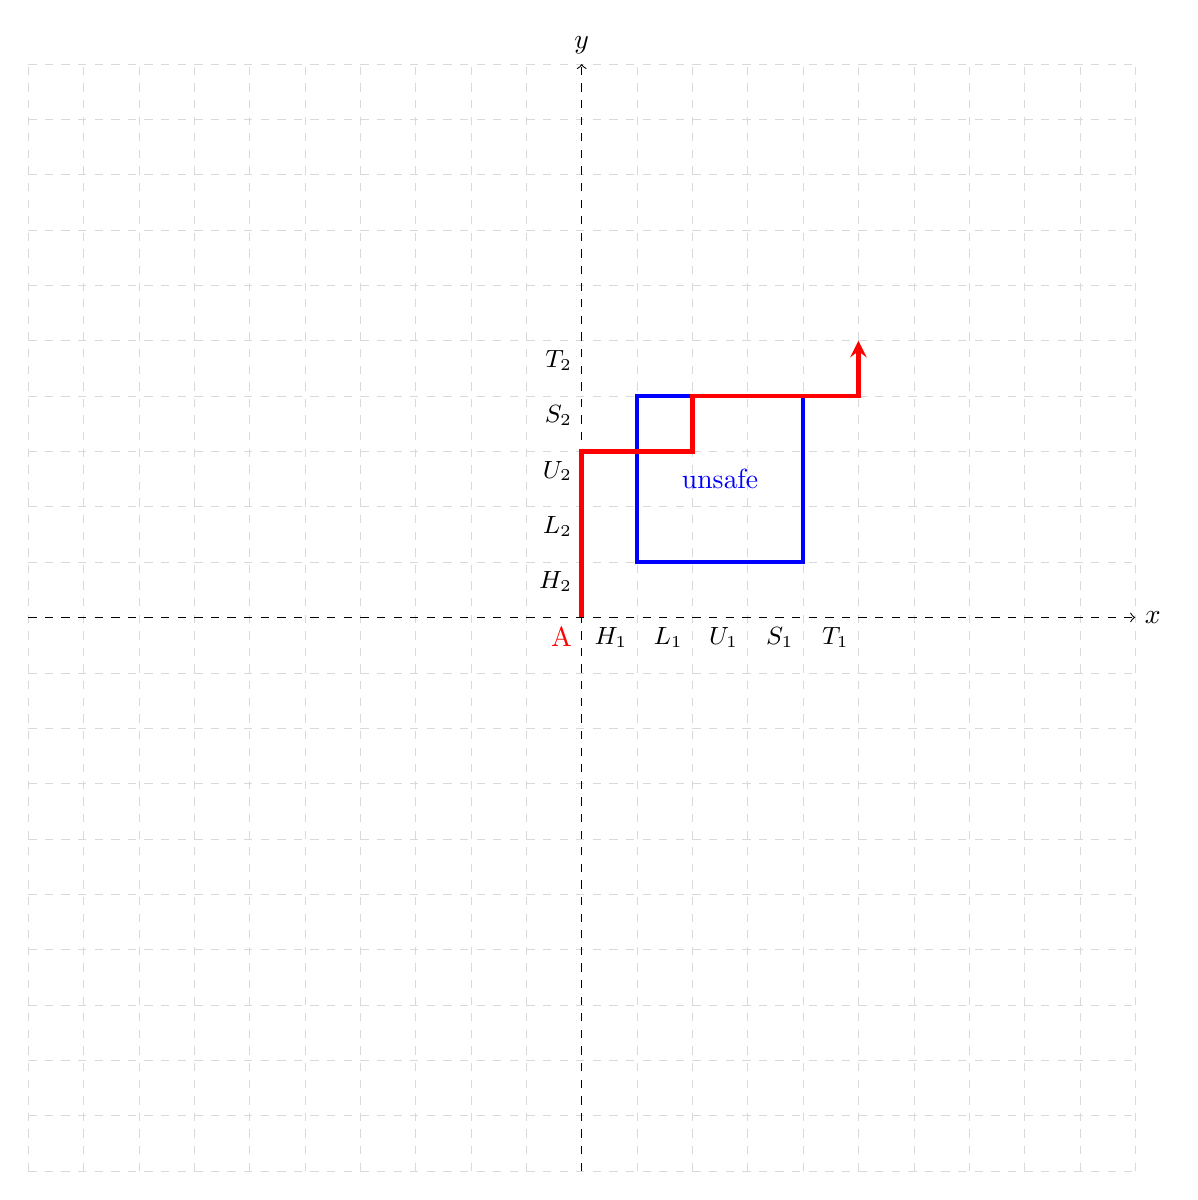
\begin{tikzpicture}[x=20pt,y=20pt]
% https://www.baeldung.com/cs/latex-define-variables
\def\axeswidth{10}
\draw[help lines, color=gray!30, dashed] (-\axeswidth,-\axeswidth) grid[step={($(1, 1) - (0, 0)$)}] (\axeswidth,\axeswidth);
\draw[->,dashed] (-\axeswidth,0)--(\axeswidth,0) node[right]{$x$};
\draw[->,dashed] (0,-\axeswidth)--(0,\axeswidth) node[above]{$y$};
% https://tex.stackexchange.com/questions/96340/how-to-place-a-textnode-at-the-center-of-a-drawn-rectangle
% https://www.overleaf.com/learn/latex/TikZ_package
% \draw[orange, very thick] (2,2) rectangle (3,3) node[pos=.5] {region k};
\draw[blue, very thick] (1,1) rectangle (4,4) node[pos=.5] {unsafe};
% \draw[red, very thick] (6,6) rectangle (7,7) node[pos=.5] {region t};

% https://tex.stackexchange.com/questions/29233/tikz-adding-text
% https://tikz.dev/tikz-shapes
% https://tex.stackexchange.com/questions/24372/how-to-add-newline-within-node-using-tikz
\node [anchor=north east,red] at (0,0) {\shortstack{A}};
\node [anchor=north east] at (1,0) {\small $H_1$};
\node [anchor=north east] at (2,0) {\small $L_1$};
\node [anchor=north east] at (3,0) {\small $U_1$};
\node [anchor=north east] at (4,0) {\small $S_1$};
\node [anchor=north east] at (5,0) {\small $T_1$};
\node [anchor=north east] at (0,1) {\small $H_2$};
\node [anchor=north east] at (0,2) {\small $L_2$};
\node [anchor=north east] at (0,3) {\small $U_2$};
\node [anchor=north east] at (0,4) {\small $S_2$};
\node [anchor=north east] at (0,5) {\small $T_2$};

% https://latexdraw.com/exploring-tikz-arrows/
% A
\draw [-stealth,ultra thick,red](0,0) -- (0,3) -- (2,3) -- (2,4) -- (5,4) -- (5,5);
\end{tikzpicture}

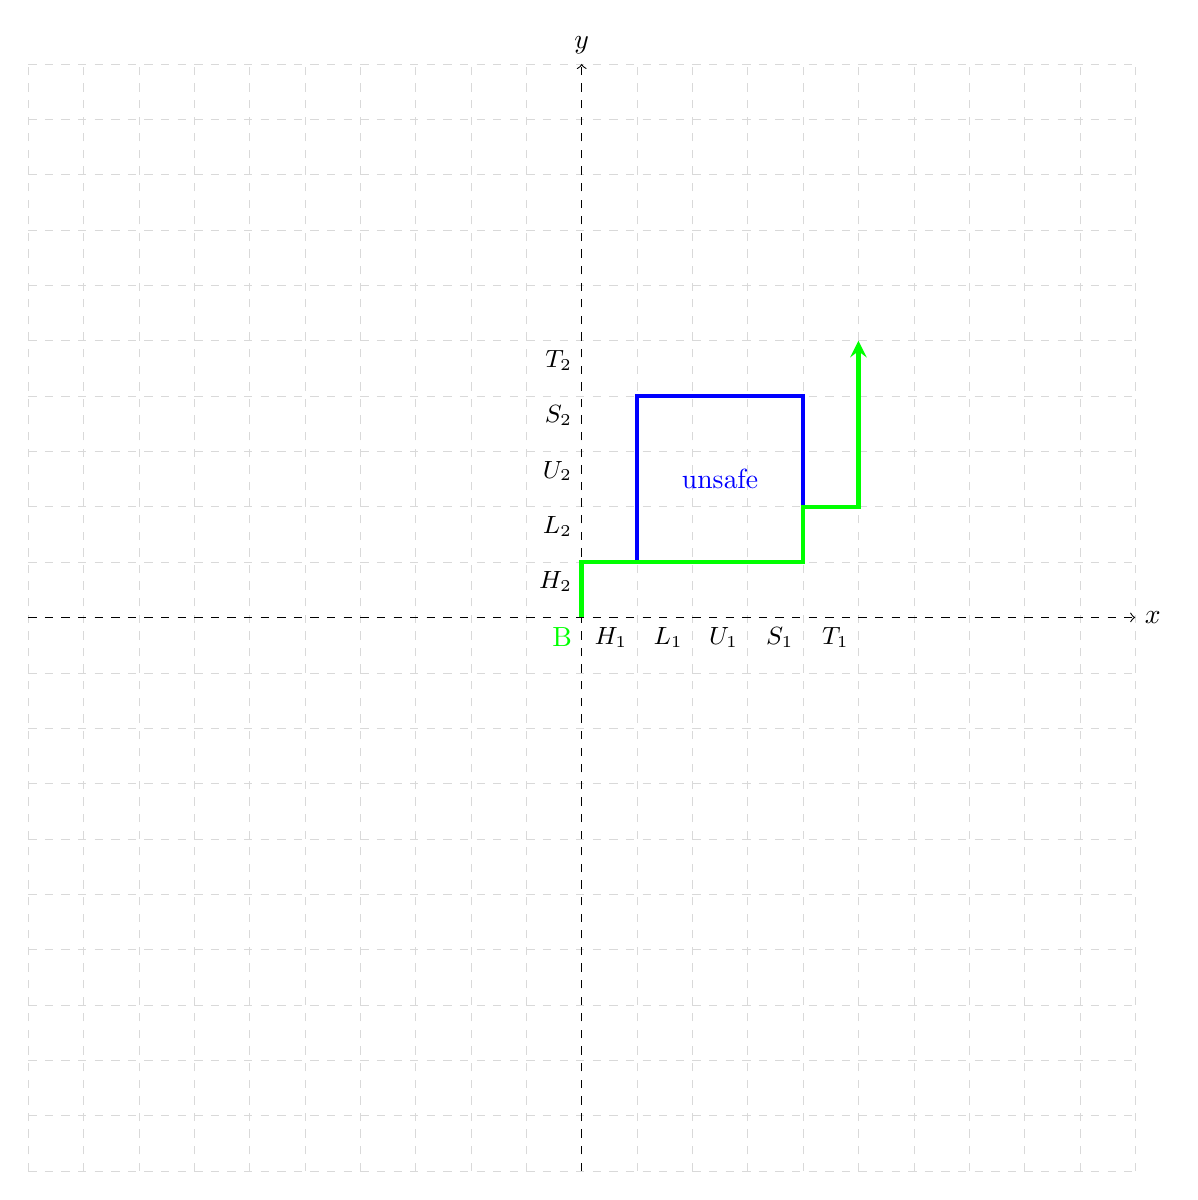
\begin{tikzpicture}[x=20pt,y=20pt]
% https://www.baeldung.com/cs/latex-define-variables
\def\axeswidth{10}
\draw[help lines, color=gray!30, dashed] (-\axeswidth,-\axeswidth) grid[step={($(1, 1) - (0, 0)$)}] (\axeswidth,\axeswidth);
\draw[->,dashed] (-\axeswidth,0)--(\axeswidth,0) node[right]{$x$};
\draw[->,dashed] (0,-\axeswidth)--(0,\axeswidth) node[above]{$y$};
% https://tex.stackexchange.com/questions/96340/how-to-place-a-textnode-at-the-center-of-a-drawn-rectangle
% https://www.overleaf.com/learn/latex/TikZ_package
% \draw[orange, very thick] (2,2) rectangle (3,3) node[pos=.5] {region k};
\draw[blue, very thick] (1,1) rectangle (4,4) node[pos=.5] {unsafe};
% \draw[red, very thick] (6,6) rectangle (7,7) node[pos=.5] {region t};

% https://tex.stackexchange.com/questions/29233/tikz-adding-text
% https://tikz.dev/tikz-shapes
% https://tex.stackexchange.com/questions/24372/how-to-add-newline-within-node-using-tikz
\node [anchor=north east,green] at (0,0) {\shortstack{B}};
\node [anchor=north east] at (1,0) {\small $H_1$};
\node [anchor=north east] at (2,0) {\small $L_1$};
\node [anchor=north east] at (3,0) {\small $U_1$};
\node [anchor=north east] at (4,0) {\small $S_1$};
\node [anchor=north east] at (5,0) {\small $T_1$};
\node [anchor=north east] at (0,1) {\small $H_2$};
\node [anchor=north east] at (0,2) {\small $L_2$};
\node [anchor=north east] at (0,3) {\small $U_2$};
\node [anchor=north east] at (0,4) {\small $S_2$};
\node [anchor=north east] at (0,5) {\small $T_2$};

% https://latexdraw.com/exploring-tikz-arrows/
% B
% B
\draw [-stealth,green,ultra thick](0,0) -- (0,1) -- (4,1) -- (4,2) -- (5,2) -- (5,5);
\end{tikzpicture}

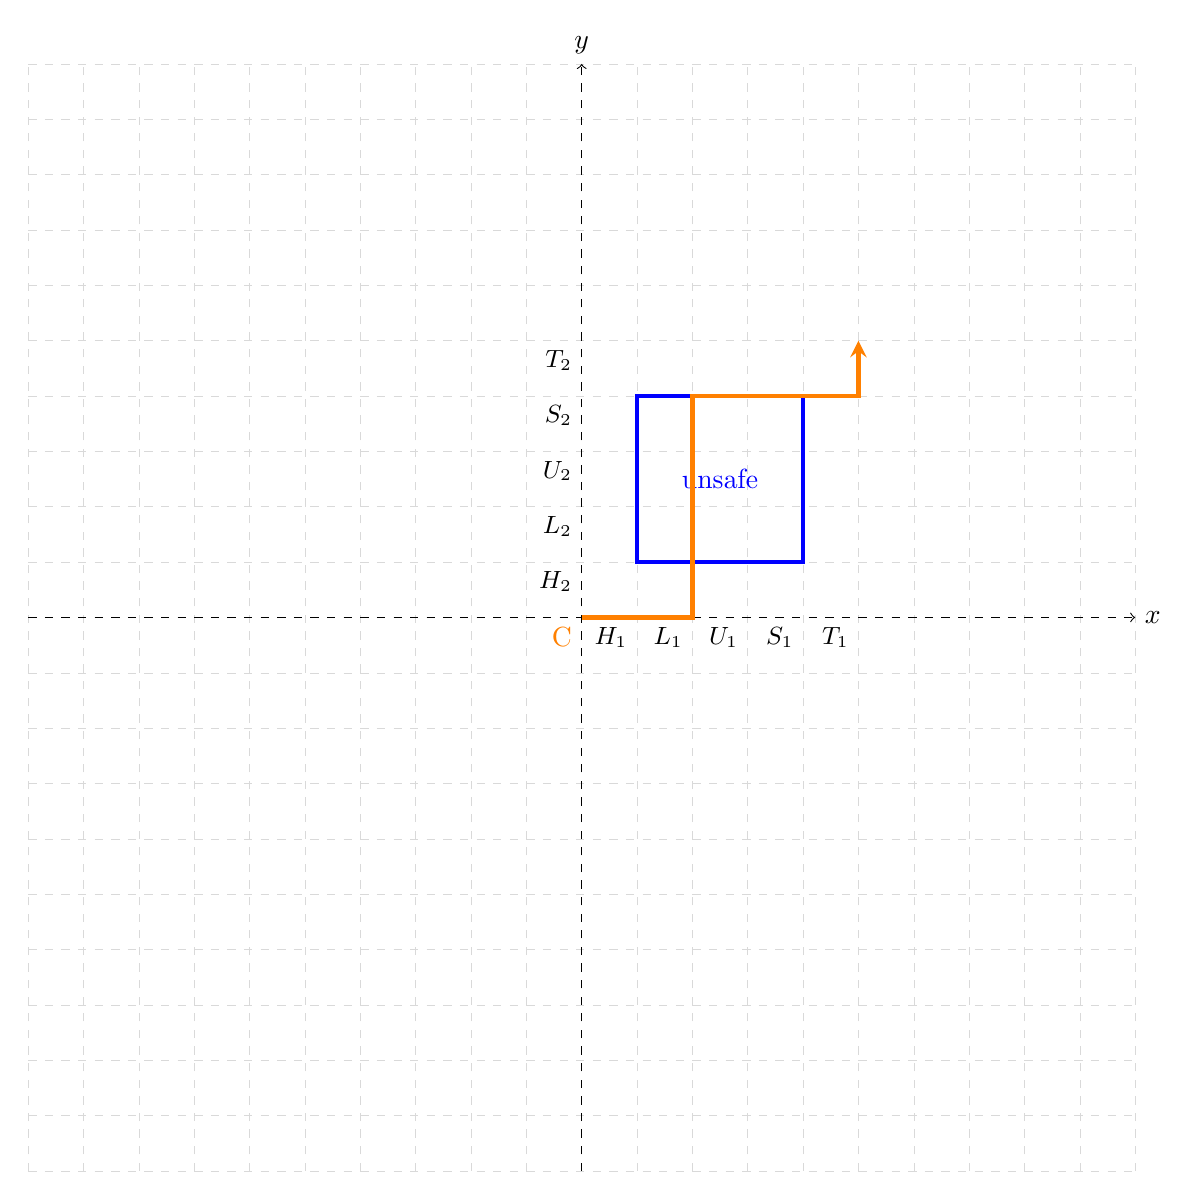
\begin{tikzpicture}[x=20pt,y=20pt]
% https://www.baeldung.com/cs/latex-define-variables
\def\axeswidth{10}
\draw[help lines, color=gray!30, dashed] (-\axeswidth,-\axeswidth) grid[step={($(1, 1) - (0, 0)$)}] (\axeswidth,\axeswidth);
\draw[->,dashed] (-\axeswidth,0)--(\axeswidth,0) node[right]{$x$};
\draw[->,dashed] (0,-\axeswidth)--(0,\axeswidth) node[above]{$y$};
% https://tex.stackexchange.com/questions/96340/how-to-place-a-textnode-at-the-center-of-a-drawn-rectangle
% https://www.overleaf.com/learn/latex/TikZ_package
% \draw[orange, very thick] (2,2) rectangle (3,3) node[pos=.5] {region k};
\draw[blue, very thick] (1,1) rectangle (4,4) node[pos=.5] {unsafe};
% \draw[red, very thick] (6,6) rectangle (7,7) node[pos=.5] {region t};

% https://tex.stackexchange.com/questions/29233/tikz-adding-text
% https://tikz.dev/tikz-shapes
% https://tex.stackexchange.com/questions/24372/how-to-add-newline-within-node-using-tikz
\node [anchor=north east,orange] at (0,0) {\shortstack{C}};
\node [anchor=north east] at (1,0) {\small $H_1$};
\node [anchor=north east] at (2,0) {\small $L_1$};
\node [anchor=north east] at (3,0) {\small $U_1$};
\node [anchor=north east] at (4,0) {\small $S_1$};
\node [anchor=north east] at (5,0) {\small $T_1$};
\node [anchor=north east] at (0,1) {\small $H_2$};
\node [anchor=north east] at (0,2) {\small $L_2$};
\node [anchor=north east] at (0,3) {\small $U_2$};
\node [anchor=north east] at (0,4) {\small $S_2$};
\node [anchor=north east] at (0,5) {\small $T_2$};

% https://latexdraw.com/exploring-tikz-arrows/
% C
\draw [-stealth,orange,ultra thick](0,0) -- (2,0) -- (2,4) -- (5,4) -- (5,5);
\end{tikzpicture}

\end{document}

% \section{Introduction}

% \end{document}
